\documentclass[10pt]{acmtrans2e}
\usepackage{hyperref}
\usepackage{amsmath}
\usepackage{amssymb}
\usepackage{amsfonts}
\usepackage{amscd}
\usepackage{amsmath}
\usepackage{latexsym}
\usepackage{graphicx}
\usepackage{geometry}
\usepackage{tikz-uml}
\usepackage{ifthen}
\usepackage{multicol}
\usepackage{paralist} % for compactitem und compactenum
% \usepackage{ellipsis}
\frenchspacing
\usepackage{nth}     % oridinal numbers: 1st, 2nd, ... by \nth{1}, \nth{2}, ...
                     % \usepackage[super]{nth} % Option 'super' not available at University
\usepackage{xspace}
\usepackage{enumitem}
\usepackage{listings}
\usepackage{epstopdf}
\usepackage{caption}
\usepackage{subcaption}
\usepackage{listings}
% MATLAB environment for source code in lstlisting
\lstloadlanguages{Matlab}
\lstset{%
float=ht, % float does not work globally..., see workaround below
basicstyle={\small\sffamily}, % alternative: ttfamily
literate=*{*}{\normalfont{*}}1, % Solution of the problem that asterik is vertically centered
columns=fullflexible, % fullflexible, flexible and fixed
frame=tb,
% language=Matlab,
upquote=true, % Simple quotes in source code are the correct ones... (otherwise MATLAB error...)
numbers=left,
numberstyle={\tiny},
showstringspaces=false,
captionpos=b, % lstlisting: define position of caption
keepspaces=true
}

\hypersetup{
  colorlinks = false,
  urlcolor = blue,
  linkcolor = blue,
  pdfauthor = {Hao Lin},
  pdfkeywords = {Consensus clustering, $K$-means, utility function, MATLAB},
  pdftitle = {User Manual for KCC---a MATLAB package for K-means-based Consensus Clustering},
  pdfsubject = {KCC package},
  pdfpagemode = UseNone
}

\geometry{
  left=4cm,
  right=4cm,
  top=4cm,
  bottom=4cm
}

\usepackage{courier}
\newcommand{\Matlab}{\textsc{Matlab}}
\newcommand{\Octave}{\textsc{Octave}}
% \newcommand{\KCC}{\textsf{KCC}\xspace}
\newcommand{\package}[1]{\textsf{#1}\xspace} % package's name: \textsf{tboxIPscatt} and dynamic space
%\newcommand{\package}[1]{\textbf{#1}}
\newcommand{\function}[1]{\textbf{\texttt{#1}}}
\newcommand{\parameter}[1]{\texttt{#1}}

\newlength{\tabcont}
\newcommand{\tab}[1]{%
\settowidth{\tabcont}{#1}%
\ifthenelse{\lengthtest{\tabcont < 1cm}}%
{\makebox[1cm][l]{#1}\ignorespaces}%
{\makebox[2cm][l]{#1}\ignorespaces}%
}%

\newcommand{\syntax}[1]{\medskip
\noindent \textbf{Syntax:} \medskip

\texttt{#1}
}

\newenvironment{inputlist}
{\vspace*{0.25cm}
\noindent \textbf{Input parameters:}
\begin{itemize}
}  
{ 
\end{itemize}
}

\newenvironment{outputlist}
{\vspace*{0.075cm}
\noindent \textbf{Output parameters:}
\begin{itemize}
}  
{ 
\end{itemize}
}

\newenvironment{remark}
{\vspace*{0.1cm}
\noindent \textbf{Discussion:} \medskip

}
{
\vspace*{0.2cm}
}

\newenvironment{example}
{\vspace*{0.1cm}
\noindent \textbf{Example:} \vspace*{0.15cm}

\setlength{\parskip}{0.5ex plus 0.5exminus 0.2 ex}
}
{\medskip
}

\newcommand{\paramitem}[2]{\item[] \tab{\texttt{#1}} \tab{: #2} }

\firstfoot{}
\runningfoot{}

\markboth{Hao Lin}{User Manual for \package{KCC}---a {MATLAB} package for K-means-based Consensus Clustering}

\title{User Manual for \package{KCC}---a {MATLAB} package for K-means-based Consensus Clustering} 

% \author{Hao Lin}
% \orcid{0000-0002-1921-3036}
% \email{linh@in.tum.de}
% \affiliation{%
%   \institution{Department of Informatics, Technical University of Munich}
%   \streetaddress{Boltzmannstr. 3}
%   \city{Garching}
%   \postcode{85748}
%   \country{Germany}
% }

% \author{Hongfu Liu}
% \email{hongfuliu@brandeis.edu}
% \affiliation{%
%   \institution{Michtom School of Computer Science, Brandeis University}
%   \streetaddress{415 South St}
%   \city{Waltham}
%   \state{MA}
%   \postcode{02453}
%   \country{USA}
% }

% \author{Junjie Wu}
% \authornote{Corresponding Author}
% \email{wujj@buaa.edu.cn}
% \affiliation{%
%   \institution{School of Economics and Management, Beihang University}
%   \streetaddress{37 Xueyuan Rd}
%   \city{Haidian District}
%   \state{Beijing}
%   \postcode{100191}
%   \country{China}
% }

% \author{Hong Li}
% \email{hong_lee@buaa.edu.cn}
% \affiliation{%
%   \institution{School of Economics and Management, Beihang University}
%   \streetaddress{37 Xueyuan Rd}
%   \city{Haidian District}
%   \state{Beijing}
%   \postcode{100191}
%   \country{China}
% }

% \author{Stephan Günnemann}
% \email{guennemann@in.tum.de}
% \affiliation{%
%   \institution{Department of Informatics, Technical University of Munich}
%   \streetaddress{Boltzmannstr. 3}
%   \city{Garching}
%   \postcode{85748}
%   \country{Germany}
% }

\author{
Hao Lin\footnote{Department of Informatics, Technical University of Munich, Germany,
\textsf{\href{mailto:linh@in.tum.de}{linh@in.tum.de}}.}, \quad
Hongfu Liu\footnote{Michtom School of Computer Science, Brandeis University, USA, \textsf{\href{mailto:hongfuliu@brandeis.edu}{hongfuliu@brandeis.edu}}.}, \quad
Junjie Wu\footnote{School of Economics and Management, Beihang University, China, \textsf{\href{mailto:wujj@buaa.edu.cn}{wujj@buaa.edu.cn}}.}, \quad
Hong Li\footnote{School of Economics and Management, Beihang University, China, \textsf{\href{mailto:hong_lee@buaa.edu.cn}{hong\_lee@buaa.edu.cn}}.}, \quad
Stephan Günnemann\footnote{Department of Informatics, Technical University of Munich, Germany, \textsf{\href{mailto:guennemann@in.tum.de}{guennemann@in.tum.de}}.}
}
\date{User Manual for \package{KCC}, updated \today}

\begin{document}

\maketitle

\vspace*{-0.5cm}

\section{Introduction}

This user manual systematically presents the usage of the \Matlab{} package on K-means-based Consensus Clustering (KCC) accompanying the following paper:
\begin{center}
\begin{minipage}{0.90\textwidth}
Hao Lin, Hongfu Liu, Junjie Wu, Hong Li, and Stephan Günnemann. 2022. Algorithm xxxx: KCC: A MATLAB Package for K-means-based Consensus Clustering. \emph{ACM Trans. Math. Softw}.
\end{minipage}
\end{center}

\noindent For package installation, you need to first unpack the compressed archive into your current directory. It consists of a \emph{source code} folder \textsf{Matlab}, a folder \textsf{userManual} with this comprehensive \emph{user manual}, and a \emph{license} file \textsf{LICENSE} indicating that the package is distributed under GNU GENERAL PUBLIC LICENSE (Version 3). Then under the \textsf{Matlab} folder, you need to add one of its subfolder, i.e., the \textsf{Src} folder, to the \Matlab{} path. The directory structure of the \textsf{Matlab} folder is described as follows.
% \setlength{\columnseprule}{0.25pt}
% \setlength{\columnsep}{10pt}
% \begin{multicols}{2}[][10mm]
\begin{compactitem}
  \item \textsf{Src} (core functions for conducting KCC)
  \begin{compactitem}
   \item \textsf{BasicCluster\_RFS.m} (function to generate BPs with RFS)
   \item \textsf{BasicCluster\_RPS.m} (function to generate BPs with RPS)
   \item \textsf{Preprocess.m} (function to prepare for consensus clustering)
   \item \textsf{KCC.m} (consensus function)
   \item \textsf{exMeasure.m} (function to compute external validity scores)
   \item \textsf{inMeasure.m} (function to compute internal validity scores)

   \item \textsf{load\_sparse.m} (auxiliary function to load input text data as a sparse matrix)
   \item \textsf{hungarian.m} (auxiliary function for cluster label assignment)
   \item \textsf{BasicCluster\_RPS\_missing.m} (auxiliary function to generate IBPs with strategy-I)
   \item \textsf{addmissing.m} (auxiliary function to generate IBPs using strategy-II)
   \item \textsf{distance\_*} (distance functions)
   \item \textsf{gClusterDistribution.m} (auxiliary function to calculate cluster distribution for BPs)
   \item \textsf{Ucompute.m, Ucompute\_miss.m} (auxiliary function for utility calculation)
   \item \textsf{gCentroid.m, gCentroid\_miss.m} (auxiliary function for centroid update)
   \item \textsf{sCentroid.m, sCentroid\_miss.m} (auxiliary function for centroid initialization)
  \end{compactitem}
  \item \textsf{Drivers} (illustrative examples)
  \begin{compactitem}
   \item \textsf{data} (input data for illustration)
   \item \textsf{demo.m} (function for KCC with different utility functions)
   \item \textsf{demoIBPI.m} (function for KCC with IBPs generated by strategy-I)
   \item \textsf{demoIBPII.m} (function for KCC with IBPs generated by strategy-II)
   \item \textsf{demoNumberBP.m} (function for KCC with varying number of BPs)
   \item \textsf{demoStrategyBP.m} (function for KCC with RFS strategy for BP generation)
   \item \textsf{demoEvacluster.m} (function for cluster evaluation and selection of $K$)
   \item \textsf{demoEvaTimeMem.m} (function for recording execution time and memory usage)
  \end{compactitem}
\end{compactitem}
% \end{multicols}

The package was developed and tested in \Matlab{} R2022a under Linux. To those without access to \Matlab{} and those who prefer to use free open source software, we also investigate the usage of \package{KCC} with \Octave{}. Generally, the Octave supports drop-in compatibility with the \Matlab{} scripts in our \package{KCC} package. To use the \package{KCC} package with \Octave{}, the users need to firstly do an additional installation step, i.e., installing the statistics and io packages on the \Octave{} command line using ``pkg install -forge statistics;'' and ``pkg install -forge io;'', respectively. Then, the users should type the commands ``pkg load statistics;'' and/or ``pkg load io;'' on the \Octave{} command line before executing the functions/scripts in the KCC package if needed. All demonstration scripts with the prefix named ``demo'' under the \textsf{Matlab/Drivers} folder have passed the test on a personal computer with GNU \Octave{} 7.1.0 and macOS 12.4.

\begin{figure*}[!bt]
\centering
\includegraphics[width=0.85\textwidth]{fig/soft.eps}
\caption{Typical program flow of \package{KCC} package.}\label{fig:soft} % \label should be placed after \caption
\end{figure*}

% Figure~\ref{fig:soft} illustrates a typical program flow of using the \package{KCC} package, which includes data preparation, basic partitions generation, consensus clustering preprocessing, consensus function, and clustering quality evaluation. We can see from Figure~\ref{fig:soft} that, in a typical flow for consensus clustering, a real-world matrix \textsf{Data} is first input to generate a basic partition matrix \textsf{IDX}. The basic partition matrix is then input to a \textsf{Preprocess} function to produce the sparse representation of $\mathcal{X}^{(b)}$, i.e., the binary matrix \textsf{binIDX}. The binary matrix \textsf{binIDX}, along with the basic partition matrix \textsf{IDX} is the input of the final consensus clustering via a $K$-means heuristic, also known as consensus function, which produces a consensus partition matrix \textsf{index}. Lastly, the clustering quality is evaluated with an \textsf{exMeasure} function, which outputs several external validity indices and a contingency matrix. We will take a detailed look at the important functions and fields in the Guides in Section~\ref{sec:guides}.

In Figure~\ref{fig:soft}, we show the package's typical workflow, which provides a quick overview for using the package. The workflow starts by inputing a real-world data matrix \textsf{Data} into the basic partition generation functions in order to generate a basic partition matrix \textsf{IDX}. The basic partition matrix is then input to a \textsf{Preprocess} function to produce a sparse representation of $\mathcal{X}^{(b)}$, i.e., the matrices, \textsf{Ki}, \textsf{sumKi}, and \textsf{binIDX}. They are then input to the final consensus clustering, i.e., the consensus function, which produces a consensus partition matrix \textsf{index}. Lastly, the clustering quality is evaluated with an \textsf{inMeasure}/\textsf{exMeasure} function, which outputs multiple internal/external validity indices.

\textcolor{blue}{\textbf{Organization of this user manual.} In Section~\ref{sec:examples}, we give some typical examples with \Matlab{} code snippets, tables and figures to help the readers to quickly understand how to work properly and effectively with the package. Next, we provide details for each of the package's available functions, such as syntax, input and output, in Section~\ref{sec:functions}.}

\section{Illustrative examples}\label{sec:examples}
\subsection{A quick introductory example for illustrating the typical workflow} \label{subsec:illexam}
\textcolor{blue}{Here we give illustrative examples with UCI and TREC data sets to show how the \package{KCC} package works following the typical workflow as previously described.}

\textbf{Importing data}. Firstly, we should import the data set into the \Matlab{} environment. For a UCI data set such as \textit{iris}, the package \package{KCC} includes two files under the \textbf{Matlab/Drivers/data} folder, i.e., \textbf{iris.dat} and \textbf{iris\_rclass.dat}, which correspond to the attribute information and ground truth cluster labels of data instances, respectively. As illustrated in Listing~\ref{lst:loaddata}, the data attributes and ground truth cluster labels can be imported with the built-in \Matlab{} function \function{load}. For ease of understanding, we also illustrate the attribute information of the \textit{iris} data set in Table~\ref{tab:iris}.
\begin{lstlisting}[caption={Using \function{load} to import data attributes and ground truth cluster labels.},label=lst:loaddata]
data = load('data/iris.dat');
true_label = load(strcat('data/', strcat('iris', '_rclass.dat')));
\end{lstlisting}

For TREC data sets such as \textit{mm}, as indicated in Listing~\ref{lst:loadsparsedata}, we use the function \function{load\_sparse} implemented in the \package{KCC} package to import the data attributes as a sparse matrix \parameter{sp\_mtx}, and use the built-in function \function{load} to import the ground truth cluster labels. The attribute matrix of the \textit{mm} data set input to \function{load\_sparse} is illustrated in Table~\ref{tab:mm_cluto}. We can see that the input attribute matrix is in a CLUTO sparse matrix format. The first line gives some meta information of the data set, which includes the number of instances $n$, the number of features $d$, and the total number of non-zero elements if recovering the data set as a $n \times d$ matrix. The file's remaining $n$ lines preserve the non-zero values of the matrix in a sparse manner~\cite{karypis2002cluto}.
\begin{lstlisting}[caption={Using \function{load\_sparse}/\function{load} to import data attributes/ground truth cluster labels.},label=lst:loadsparsedata]
[sp_mtx, n, m, count] = load_sparse('data/mm.mat');
data = sp_mtx;
true_label = load(strcat('data/',strcat('mm', '_rclass.dat')));
\end{lstlisting}

\begin{table*}[!tb]
\centering
\scriptsize    
    \begin{subtable}{.5\linewidth}
      \centering
        \begin{tabular}{ccccc}
                & $attr_1$ & $attr_2$ & $attr_3$ & $attr_4$ \\ \cline{2-5}
        $data_1$   & \multicolumn{1}{ |c }{5.1}   & 3.5   & 1.4   & \multicolumn{1}{ c| }{0.2}   \\
        $data_2$   & \multicolumn{1}{ |c }{4.9}   & 3.0   & 1.4   & \multicolumn{1}{ c| }{0.2}   \\
        $data_3$   & \multicolumn{1}{ |c }{4.7}   & 3.2   & 1.3   & \multicolumn{1}{ c| }{0.2}   \\
        %$data_4$   & \multicolumn{1}{ |c }{4.6}   & 3.1   & 1.5   & \multicolumn{1}{ c| }{0.2}    \\
        $\vdots$   & \multicolumn{1}{ |c }{$\vdots$}   & $\vdots$   & $\vdots$   & \multicolumn{1}{ c| }{$\vdots$}  \\
        $data_{150}$ & \multicolumn{1}{ |c }{5.9}   & 3.0   & 5.1   & \multicolumn{1}{ c| }{1.8}  \\ \cline{2-5}
        \end{tabular}
        \caption{A $n \times d$ attribute matrix for \textit{iris} data set, \\ where $n = 150$ and $d = 4$.}\label{tab:iris}
    \end{subtable}%
    \begin{subtable}{.5\linewidth}
      \centering
        \begin{tabular}{c|ccccc|}
        \cline{2-6}
        & 2521 & 126373 & 490062 &     &    \\
        $data_1$ & 556  & 1  & $\dots$ & 238  & 1  \\
        $data_2$ & 755  & 1  & $\dots$ & 195   & 1   \\
        $data_3$ & 2202 & 2  & $\dots$ & 7848  & 1   \\
        $\vdots$ & $\vdots$  & $\vdots$ & $\vdots$ & $\vdots$   & $\vdots$ \\
        $data_{2521}$ & 595  & 1  & $\dots$ & 20246 & 3  \\ \cline{2-6}
        \end{tabular}
        \caption{A $n \times d$ attribute matrix for \textit{mm} data set, \\ where $n = 2521$ and $d = 126373$.} \label{tab:mm_cluto}
    \end{subtable} 
    \caption{Illustration of the data attribute matrix for two data sets.}
\end{table*}

\begin{table*}[!bt]
\centering
\scriptsize
\begin{tabular}{cccccccccccc}
        & $BP_1$ & $BP_2$ & $BP_3$ & $BP_4$ & $BP_5$ & $BP_6$ & $BP_{7}$ & $BP_{8}$ & $BP_{9}$ & $\dots$ & $BP_{100}$ \\ \cline{2-12}
$data_1$   & \multicolumn{1}{ |c }{1}   & 1   & 1 & 4 & 7 & 4 & 6 & 1 & 10 & $\dots$ & \multicolumn{1}{ c| }{7}   \\
$data_2$   & \multicolumn{1}{ |c }{1}   & 8   & 4 & 3 & 1 & 2 & 4 & 1 & 1 & $\dots$ & \multicolumn{1}{ c| }{7}   \\
$data_3$   & \multicolumn{1}{ |c }{1}   & 8   & 10 & 3 & 1 & 2 & 4 & 1 & 6 & $\dots$ & \multicolumn{1}{ c| }{7}   \\
$data_4$   & \multicolumn{1}{ |c }{1}   & 8   & 10 & 3 & 1 & 2 & 4 & 1 & 6 & $\dots$ & \multicolumn{1}{ c| }{7}   \\
$data_5$   & \multicolumn{1}{ |c }{1}   & 1   & 1 & 4 & 7 & 4 & 6 & 1 & 10 & $\dots$ & \multicolumn{1}{ c| }{7}   \\
$\vdots$   & \multicolumn{1}{ |c }{$\vdots$}   & $\vdots$   & $\vdots$  & $\vdots$ & $\vdots$ & $\vdots$ & $\vdots$ & $\vdots$ & $\vdots$ & $\vdots$ & \multicolumn{1}{ c| }{$\vdots$}  \\
$data_{150}$ & \multicolumn{1}{ |c }{2}   & 3   & 3  & 1 & 8 & 1 & 5 & 2 & 11 & $\dots$ & \multicolumn{1}{ c| }{8}  \\ \cline{2-12}
\end{tabular}
\caption{A $n \times r$ basic partition matrix \parameter{IDX} for the \textit{iris} data set, where $n = 150$ and $r = 100$.}\label{tab:bpmatrix}
\end{table*}

\textbf{Generating basic partitions}. As indicated in Figure~\ref{fig:soft}, we should then generate basic partitions (BPs). Concretely, we can utilize the \function{BasicCluster\_RPS} function to produce BPs with Random Parameter Selection (RPS) strategy. We set the number of BPs to 100~\cite{luo2011consensus,liu2016infinite}, because this setting can usually produce good consensus clustering results. For the data set \textit{iris}, we use squared euclidean distance as the distance metric of clustering algorithm to generate BPs, while we use cosine distance for the \textit{mm} data set. The code snippet is shown in Listing~\ref{lst:producebps}. We also illustrate the obtained basic partition matrix \parameter{IDX} for the \textit{iris} data set in Table~\ref{tab:bpmatrix}. Each entry in \parameter{IDX} represents a cluster label that the corresponding data object is assigned to in a basic partition. 
\begin{lstlisting}[caption={Using \function{BasicCluster\_RPS} to generate BPs.},label=lst:producebps]
IDX = BasicCluster_RPS(data, 100, 3, 'sqEuclidean', 1); % for iris
IDX = BasicCluster_RPS(data, 100, 2, 'cosine', 1); % for mm
\end{lstlisting}

For further consideration of efficiency, we can also utilize the multicore-processor architecture to reduce the execution time of the \package{KCC} package. In fact, the parallel 'for-loop' function, i.e., \function{parfor}, in \Matlab{} \package{Parallel Computing Toolbox} can be employed in the \package{KCC} package for the computation acceleration purpose. Listing~\ref{lst:parforproducebps} demonstrates how the \function{parfor} function can be used to help accelerate the generation process of basic partitions in the \function{BasicCluster\_RPS} function.
\begin{lstlisting}[caption={Using \function{parfor} to accelerate the process of generating BPs.},label=lst:parforproducebps]
parfor i = 1:r
    IDX(:, i) = kmeans(Data, Ki(i), 'distance', dist, 'emptyaction', 'singleton', 'replicates', 1);
end
\end{lstlisting}

\textbf{Preprocessing data and conducting consensus function}. As a next step of the workflow in Figure~\ref{fig:soft}, the function \function{RunKCC} is executed with the basic partition matrix \parameter{IDX} as the input. An illustrated code to conduct consensus clustering on the \textit{iris} data set with $U_h$ utility function and $K=3$ is shown in Listing~\ref{lst:consensusclustering}. The \function{RunKCC} is composed of two key steps, which involves executing the \function{Preprocess} function to prepare input for consensus clustering and executing the core function \function{KCC} 10 times to find the best consensus partition \parameter{pi\_index}, which has the best objective function value.
\begin{lstlisting}[caption={Using \function{RunKCC} to conduct consensus clustering.},label=lst:consensusclustering]
K = 3;
U = {'U_h', 'std', []};
r = size(IDX, 2);
w = ones(r, 1);
rep = 10;
maxIter = 40;
minThres = 1e-5;
utilFlag = 1;
[pi_sumbest, pi_index, ~, ~~, ~~~] = RunKCC(IDX, K, U, w, rep, maxIter, minThres, utilFlag);
\end{lstlisting}

\textbf{Evaluating clustering quality}. As a last step of the workflow in Figure~\ref{fig:soft}, users can utilize the external validity metrics to evaluate the clustering quality with the \function{exMeasure} function in \package{KCC} package. The code to launch the \function{exMeasure} function is shown in Listing~\ref{lst:evaqualityexternal}, which saves values of five external validity measurements to a result matrix file for further comparison.
\begin{lstlisting}[caption={Using \function{exMeasure} to evaluate the clustering quality.},label=lst:evaqualityexternal]
[Acc, Rn, NMI, VIn, VDn, labelnum, ncluster, cmatrix] = exMeasure(pi_index, true_label);
filename = strcat('iris', strcat('_', lower(U{1, 1})));
filename = strcat(filename, strcat('_', lower(U{1, 2})));
if ~isempty(U{1, 3})
    filename = strcat(filename, strcat('_', num2str(lower(U{1, 3}))));
end
filename = strcat(filename, '.mat');
save(filename, 'Acc', 'VIn', 'VDn', 'Rn', 'NMI');
\end{lstlisting}

When the ground truth cluster labels are not available in real-world settings, we can utilize the internal validity metrics to evaluate a clustering with the \function{inMeasure} function in \package{KCC} package. An illustrated code snippet is shown in Listing~\ref{lst:evaqualityinternal}.
\begin{lstlisting}[caption={Using \function{inMeasure} to evaluate the clustering quality.},label=lst:evaqualityinternal]
[Distortion, Silhouette, CH] = inMeasure(X, cluster, k);
\end{lstlisting}

\subsection{An illustrative example of choosing effective and efficient utility function}\label{subsec:example1}
\textcolor{blue}{Choosing effective and efficient utility function is a common need for the \package{KCC} package in practical clustering applications. In order to achieve this purpose, the \package{KCC} package provides demonstration scripts to compare clustering quality and efficiency with different utility functions on 11 real-world data sets from UCI and TREC repositories.}

For effectiveness comparison, the \package{KCC} package provides the script \textbf{Matlab/Drivers/demo.m}. We briefly explain the main steps in this illustration. The first step utilizes an RPS strategy to generate basic partitions, which calls the \function{BasicCluster\_RPS} function. The next step applies the \function{RunKCC} function to the obtained basic partition matrix to obtain the consensus partition. This step also involves executing consensus clustering with 10 different utility functions, namely $U_c$, $U_H$, $U_{cos}$, $U_{L_5}$, $U_{L_8}$ and their corresponding normalized versions $NU_x$. Then the script conducts clustering quality evaluation and reports five external validity indices, including $CA$, $NMI$, $R_n$, $VI_n$ and $VD_n$. For robustness concern, the script conducts the \function{RunKCC} function 10 times to obtain the average validity values. In the following, we show the most important code snippet for this illustration.
\begin{lstlisting}[caption={Using \function{demo.m} to evaluate the clustering quality of \package{KCC} with different utility functions.},label=lst:evaqualityutility]
U_array = {{'U_H','std',[]} {'U_H','norm',[]} {'U_c','std',[]} {'U_c','norm',[]} {'U_cos','std',[]} 
{'U_cos','norm',[]} {'U_lp','std',[5]} {'U_lp','norm',[5]} {'U_lp','std',[8]} {'U_lp','norm',[8]}};
IDX = BasicCluster_RPS(data, r, K, dist_of_basic_cluster, randKi);
output_foldername='ResultDemo/';
mkdir ResultDemo;

for uidx = 1:length(U_array)
    avgAcc = 0;
    avgRn = 0;
    avgNMI = 0;
    avgVIn = 0;
    avgVDn = 0;
    U = U_array{1,uidx};
    for num = 1 : 10
        [pi_sumbest,pi_index,pi_converge,pi_utility,~] = RunKCC(IDX,K,U,w,rep,maxIter,minThres,utilFlag);
        [Acc, Rn, NMI, VIn, VDn, labelnum, ncluster, cmatrix] = exMeasure(pi_index, true_label);
        avgAcc = avgAcc + Acc;
        avgRn = avgRn + Rn;
        avgNMI = avgNMI + NMI;
        avgVIn = avgVIn + VIn;
        avgVDn = avgVDn + VDn;
    end
    avgAcc = avgAcc / num;
    avgRn = avgRn / num;
    avgNMI = avgNMI / num;
    avgVIn = avgVIn / num;
    avgVDn = avgVDn / num;
    filename = strcat([output_foldername '/' datafile],strcat('_',lower(U{1,1})));
    filename = strcat(filename,strcat('_',lower(U{1,2})));
    if ~isempty(U{1,3})
        filename = strcat(filename,strcat('_',num2str(lower(U{1,3}))));
    end
    filename1 = strcat(filename,'.mat');
    save(filename1,'avgAcc', 'avgVIn', 'avgVDn', 'avgRn', 'avgNMI');
end
\end{lstlisting}

\begin{table*}[!bt]
\centering
\scriptsize
\resizebox{\textwidth}{!}{
\begin{tabular}{c|cccccccccc}
\hline
& $U_c$ & $U_H$ & $U_{cos} $ &  $U_{L5}$  &  $U_{L8}$   &   $NU_c$   &  $NU_H$   &   $NU_{cos} $   &  $NU_{L5}$  &  $NU_{L8}$ \\ \hline
\textit{breast\_w} & 0.6403 & 0.9624 & 0.7172 & 0.6820 & 0.6896 & 0.6260 & \textbf{0.9639} &  0.6838 &  0.6820 &  0.6820 \\
\textit{ecoli} & 0.5639 & 0.5789 & 0.5651 & 0.5756 & 0.5590 &  0.5831 & 0.5578 & \textbf{0.5880} &  0.5605 & 0.5657 \\
\textit{iris} & 0.8940 & 0.8973 & \textbf{0.9000} & \textbf{0.9000} & 0.8940 & 0.8933 &  0.8907 & \textbf{0.9000} & \textbf{0.9000} & 0.8880\\
\textit{pendigits} & 0.6526 & 0.6584 & \textbf{0.6837} & 0.6422 & 0.6520 & 0.5947 & 0.6443 & 0.6833 & 0.6600 & 0.6533\\
\textit{satimage} & 0.5829  & 0.6571      & 0.6149  & 0.6060   & 0.6290 &  0.5229  &  0.6425   &  \textbf{0.6594} &  0.6006 &  0.5597 \\ 
\textit{dermatology} &  0.2913  &  \textbf{0.3128}      & 0.2729  & 0.2701   &  0.2723 & 0.3075  & 0.2975   & 0.2802 &  0.2760 & 0.2899 \\ 
\textit{wine} & 0.5135  & \textbf{0.5247}      &  0.5180  & 0.5112   & 0.5112 & 0.5208  & 0.5079   & 0.5219 & 0.5157 & 0.5152 \\
\textit{mm} & 0.9337  & 0.9497      & 0.9532  & 0.9336   & \textbf{0.9551} &  0.7797  & 0.9495   & 0.9415 & 0.9439 & 0.9093 \\
\textit{reviews} & 0.6153  & 0.6593      & 0.6313  & 0.6407   & 0.6569 & 0.6086  & \textbf{0.6698}   & 0.6030 & 0.6353 &  0.6198 \\
\textit{la12} & 0.4626  & 0.4912      &  \textbf{0.5064}  & 0.4755   & 0.4690 & 0.4349  & 0.4890   & 0.4853 & 0.4491 & 0.4476 \\
\textit{sports} & 0.4497  & \textbf{0.4858}      & 0.4715  & 0.4642   & 0.4502 &  0.4592  & 0.4584   & 0.4764 & 0.4693 & 0.4461  \\ \hline
% score & 10.1005 & \textbf{10.8881} & 10.4084 & 10.2111 & 10.2454 & 9.8011 & 10.6775 & 10.4243 & 10.1918 & 10.0489 \\
score & 0.9182 & \textbf{0.9898} & 0.9462 & 0.9283 & 0.9314 & 0.8910 & 0.9707 & 0.9477 & 0.9265 & 0.9135 \\
\hline
\end{tabular}}
\caption{Clustering quality of \package{KCC} with different utility functions in terms of $CA$.} \label{tab:validity_ca1}
\end{table*}

\begin{table*}[!bt]
\centering
\scriptsize
\resizebox{\textwidth}{!}{
\begin{tabular}{c|cccccccccc}
\hline
& $U_c$ & $U_H$ & $U_{cos} $ &  $U_{L5}$  &  $U_{L8}$   &   $NU_c$   &  $NU_H$   &   $NU_{cos} $   &  $NU_{L5}$  &  $NU_{L8}$ \\ \hline
\textit{breast\_w} & 0.2430 & 0.7558 & 0.2575 &  0.2024 & 0.1998 & 0.2326 & \textbf{0.7690} &  0.1850 & 0.2024 & 0.2024 \\
\textit{ecoli} & 0.5809 &  0.5941 & 0.5861 & 0.5911 & 0.5855 & 0.5937 & 0.5922 &  \textbf{0.5952} & 0.5839 &  0.5916 \\
\textit{iris} & 0.7905 &  0.7937 & \textbf{0.7981} & \textbf{0.7981} & 0.7905 & 0.7908 &  0.7767 & \textbf{0.7981} & \textbf{0.7981} & 0.7829\\
\textit{pendigits} & 0.6978 & 0.6775 & \textbf{0.7194} & 0.6756 & 0.6663 & 0.6732 & 0.6749 & 0.7062 & 0.6816 & 0.6670\\
\textit{satimage} & 0.5388  & 0.5747      & 0.5695  & 0.5695   & 0.5839 & 0.4699  &  0.5790   & \textbf{0.5840} &  0.5469 &  0.5273 \\ 
\textit{dermatology} &  0.1211  & \textbf{0.1417}      & 0.1031  & 0.0990   &  0.0916 & 0.1395  & 0.1328   & 0.1238 & 0.0955 & 0.1083 \\ 
\textit{wine} & 0.1675  & 0.1697      & 0.1689  & 0.1669   & 0.1519 & 0.1697  & 0.1511   & \textbf{0.1701} & 0.1682 & 0.1680 \\
\textit{mm} & 0.6741  & 0.7249      & 0.7338  & 0.6501   &  \textbf{0.7487} & 0.3531  & 0.7211   &  0.6924 & 0.7028 &  0.5949 \\
\textit{reviews} & 0.4879  & 0.5347     &  0.5052  &  0.5375   & \textbf{0.5575} & 0.4538  & 0.5467   &  0.4765 & 0.5147 & 0.5091 \\
\textit{la12} & 0.2646  & \textbf{0.3371}      & 0.3095  & 0.2882   &  0.2764 &  0.2256  & 0.3234   & 0.2911 & 0.2515 &  0.2630 \\
\textit{sports} & 0.4406  & 0.4641      & 0.4531  & \textbf{0.4754}   & 0.4715 &  0.4319  & 0.4499   & 0.4693 & 0.4563 & 0.4472  \\ \hline
% score & 9.5016 & \textbf{10.8025} & 9.7728 & 9.5378 & 9.5112 & 8.8767 & 10.5727 & 9.7261 & 9.3587 & 9.2487 \\
score    & 0.8638 &\textbf{0.9820} & 0.8884 & 0.8671 & 0.8647 & 0.8070 & 0.9612 & 0.8842 & 0.8508 & 0.8408\\
\hline
\end{tabular}}
\caption{Clustering quality of \package{KCC} with different utility functions in terms of $NMI$.} \label{tab:validity_nmi1}
\end{table*}

\begin{table*}[!bt]
\centering
\scriptsize
\resizebox{\textwidth}{!}{
\begin{tabular}{c|cccccccccc}
\hline
& $U_c$ & $U_H$ & $U_{cos} $ &  $U_{L5}$  &  $U_{L8}$   &   $NU_c$   &  $NU_H$   &   $NU_{cos} $   &  $NU_{L5}$  &  $NU_{L8}$ \\ \hline
\textit{breast\_w} & 0.0687  &  0.8537   &  0.2104    &  0.1283   & 0.1391 & 0.0495  &  \textbf{0.8597}   & 0.1307   &  0.1283 & 0.1283 \\
\textit{ecoli} & 0.3970  & 0.4230    & 0.4021    & 0.4128   & 0.4021 & 0.4213 &  0.4119  & \textbf{0.4342}   & 0.4007 & 0.4110  \\
\textit{iris} & 0.7352 & 0.7445   & \textbf{0.7455}   & \textbf{0.7455}   & 0.7352 & 0.7323  & 0.7287   &  \textbf{0.7455} &  \textbf{0.7455} & 0.7249  \\
\textit{pendigits} & 0.4799  & 0.5236   & \textbf{0.5662}    & 0.5073 & 0.5010 & 0.3996  & 0.5084 & 0.5551   & 0.5130 & 0.4961 \\
\textit{satimage} & 0.3989  & \textbf{0.5018}     & 0.4663  & 0.4650   & 0.4790 & 0.2704  & 0.4908   & 0.4958 & 0.4319 &  0.3955  \\ 
\textit{dermatology} &  0.0428  & \textbf{0.0553}      & 0.0305  &  0.0259   & 0.0275 & 0.0537  & 0.0442   & 0.0419 & 0.0285 & 0.0352  \\ 
\textit{wine} & 0.1454  & \textbf{0.1497}      & 0.1471  & 0.1447   &  0.1375 & 0.1480  & 0.1355   & 0.1484 & 0.1461 & 0.1459  \\
\textit{mm} & 0.7564  & 0.8092      & 0.8215  &  0.7522   & \textbf{0.8284} & 0.3454  & 0.8081   &  0.7799 & 0.7893 & 0.6791  \\
\textit{reviews} & 0.4231  & 0.5193      & 0.4797  & 0.4877   & 0.5305 & 0.3738  & \textbf{0.5334}   & 0.4403 & 0.4821 & 0.4625  \\
\textit{la12} & 0.2046  & 0.2671      & \textbf{0.2770}  & 0.2344  &  0.2397 & 0.1574  & 0.2436   & 0.2449 & 0.2059 & 0.2063  \\
\textit{sports} &  0.2639  & 0.3193     & 0.2989  & 0.3210  & 0.3229 & 0.2387  & 0.3002   & \textbf{0.3283} & 0.3081 & 0.3038 \\ \hline
% score & 8.6169 & \textbf{10.7779} & 9.4357 & 9.0039 & 9.1727 & 7.6275 & 10.2758 & 9.5205 & 8.8686 & 8.7007 \\
score     & 0.7834 & \textbf{0.9798} & 0.8578 & 0.8185 & 0.8339 & 0.6934 & 0.9342 & 0.8655 & 0.8062 & 0.7910\\
\hline
\end{tabular}}
\caption{Clustering quality of \package{KCC} with different utility functions in terms of $R_n$.} \label{tab:validity_rn1}
\end{table*}

\begin{table*}[!bt]
\centering
\scriptsize
\resizebox{\textwidth}{!}{
\begin{tabular}{c|cccccccccc}
\hline
& $U_c$ & $U_H$ & $U_{cos} $ &  $U_{L5}$  &  $U_{L8}$   &   $NU_c$   &  $NU_H$   &   $NU_{cos} $   &  $NU_{L5}$  &  $NU_{L8}$ \\ \hline
\textit{breast\_w} & 0.7572 &  0.2442 &  0.7425 & 0.7977 & 0.8003 & 0.7677 & \textbf{0.2310} & 0.8151 & 0.7977 &  0.7977 \\
\textit{ecoli} & 0.4215 & 0.4079 & 0.4164 &  0.4113 & 0.4169 & 0.4083 & 0.4099 & \textbf{0.4072} & 0.4184 &  0.4109 \\
\textit{iris} & 0.2096 & 0.2064 & \textbf{0.2020} &  \textbf{0.2020} & 0.2096 & 0.2093 & 0.2234 &  \textbf{0.2020} & \textbf{0.2020} & 0.2172\\
\textit{pendigits} & 0.3032 & 0.3227 & \textbf{0.2808} &  0.3247 & 0.3340 &  0.3289 & 0.3254 & 0.2940 &  0.3187 & 0.3333\\
\textit{satimage} & 0.4613  & 0.4253      & 0.4305  & 0.4306   & \textbf{0.4161} & 0.5311  &  0.4210   &  \textbf{0.4161} & 0.4532 & 0.4727 \\ 
\textit{dermatology} & 0.8790  & \textbf{0.8584}      & 0.8970  &  0.9010   & 0.9084 & 0.8605  & 0.8672   & 0.8762 & 0.9045 &  0.8917 \\ 
\textit{wine} & 0.8325  & 0.8303      & 0.8311  & 0.8331   & 0.8481 & 0.8303  & 0.8489   & \textbf{0.8299} &  0.8318 & 0.8320 \\
\textit{mm} &  0.3259  & 0.2752      & 0.2662  & 0.3499   & \textbf{0.2513} & 0.6505  & 0.2789   & 0.3077 & 0.2972 & 0.4052 \\
\textit{reviews} & 0.5125  & 0.4660      & 0.4956  & 0.4631   & \textbf{0.4433} & 0.5465  & 0.4539   & 0.5242 & 0.4857 & 0.4915 \\
\textit{la12} & 0.7358  & \textbf{0.6630}      &  0.6905  & 0.7119   & 0.7236 & 0.7754  & 0.6767   &  0.7090 & 0.7485 &  0.7370 \\
\textit{sports} &  0.5612  &  0.5392      & 0.5497  & \textbf{0.5278}   &  0.5315 & 0.5691  &  0.5534  & 0.5339 & 0.5467 & 0.5555 \\ \hline
% score & 9.9657 & \textbf{8.9595} & 9.5933 & 9.8457 & 9.7563 & 10.7575 & 9.0819 & 9.7609 & 9.9302 & 10.2242 \\
score       & 0.9060 & \textbf{0.8145} & 0.8721 & 0.8951 & 0.8869 & 0.9780 & 0.8256 & 0.8874 & 0.9027 & 0.9295\\
\hline
\end{tabular}}
\caption{Clustering quality of \package{KCC} with different utility functions in terms of $VI_n$.} \label{tab:validity_vin1}
\end{table*}

\begin{table*}[!bt]
\centering
\scriptsize
\resizebox{\textwidth}{!}{
\begin{tabular}{c|cccccccccc}
\hline
& $U_c$ & $U_H$ & $U_{cos} $ &  $U_{L5}$  &  $U_{L8}$   &   $NU_c$   &  $NU_H$   &   $NU_{cos} $   &  $NU_{L5}$  &  $NU_{L8}$ \\ \hline
\textit{breast\_w} & 0.9511 & 0.1087 & 0.7664 & 0.8541 & 0.8378 & 0.9720 & \textbf{0.1041} & 0.8500 &  0.8541 & 0.8541 \\
\textit{ecoli} & 0.4312 & 0.4323 & 0.4279 & \textbf{0.4148} & 0.4278 & 0.4161 & 0.4248 & 0.4173 & 0.4262 & 0.4270\\
\textit{iris} & 0.1729 & 0.1675 &  \textbf{0.1622} & \textbf{0.1622} & 0.1729 &  0.1739 & 0.1779 & \textbf{0.1622} &  \textbf{0.1622} & 0.1837 \\
\textit{pendigits} & 0.3380 & 0.3386 &  \textbf{0.3006} &  0.3418 & 0.3467 &  0.3859 & 0.3444 & 0.3133 & 0.3410 & 0.3582\\
\textit{satimage} & 0.4549  & \textbf{0.3829}      & 0.4184  & 0.4198   & 0.4036 & 0.5686  & 0.3980   & 0.3859 & 0.4487 & 0.4805 \\ 
\textit{dermatology} &  0.9170  & \textbf{0.8877}      &  0.9342  &  0.9370   & 0.9328 & 0.9000  & 0.8977   & 0.9205 & 0.9293 & 0.9246 \\ 
\textit{wine} & 0.7516  & \textbf{0.7399}      &  0.7526  &  0.7512   & 0.7570 & 0.7531  & 0.7571  & 0.7534 & 0.7521 &  0.7520 \\
\textit{mm} & 0.1546  &  0.1083     & 0.1016  &  0.1504   & \textbf{0.0968} & 0.5553  & 0.1091   & 0.1254 & 0.1244 &  0.2181 \\
\textit{reviews} & 0.4749  & 0.4042      & 0.4089  & 0.4094   & 0.3866 & 0.4915  & \textbf{0.3799}   & 0.4496 & 0.4315 & 0.4380 \\
\textit{la12} & 0.7167  & 0.6286      & \textbf{0.6270}  & 0.6695   & 0.6765 & 0.7898  & 0.6485   & 0.6725 & 0.7091 & 0.7066 \\
\textit{sports} & 0.6014  & 0.5335      &  0.5512  & 0.5342   & 0.5372 & 0.6236  & 0.5555   & \textbf{0.5295} & 0.5360 &  0.5644 \\ \hline
% score & 9.6809 & \textbf{8.1680} & 8.8598 & 9.1455 & 9.0752 & 10.8644 & 8.2900 & 9.0320 & 9.2648 & 9.7034 \\
score       & 0.8801 & \textbf{0.7425} & 0.8054 & 0.8314 & 0.8250 & 0.9877 & 0.7536 & 0.8211 & 0.8423 & 0.8821\\
\hline
\end{tabular}}
\caption{Clustering quality of \package{KCC} with different utility functions in terms of $VD_n$.} \label{tab:validity_vdn1}
\end{table*}

\begin{table*}[!bt]
\centering
\scriptsize
\resizebox{\textwidth}{!}{
\begin{tabular}{c|cccccccccc}
\hline
& $U_c$ & $U_H$ & $U_{cos} $ &  $U_{L5}$  &  $U_{L8}$   &   $NU_c$   &  $NU_H$   &   $NU_{cos} $   &  $NU_{L5}$  &  $NU_{L8}$ \\ \hline
\textit{breast\_w}   & 0.83    & 1.95    & 0.72   & 0.88    & 0.76   & 0.82   & 0.99    & \textbf{0.64}   & 0.76   & 0.86   \\
\textit{ecoli}       & 1.61    & 3.50    & 1.24   & 1.67    & 1.51   & \textbf{1.16}   & 2.06    & 1.23   & 1.50   & 1.40   \\
\textit{iris}        & 2.00    & 7.06    & 1.61   & 1.51    & 1.51   & 1.49   & 3.39    & 1.48   & \textbf{1.46}   & 1.48   \\
\textit{pendigits}   & \textbf{10.55}   & 12.87   & 11.45  & 13.84   & 11.87  & 11.39  & 13.00   & 11.19  & 14.01  & 13.12  \\
\textit{satimage}    & 1.25    & 1.80    & \textbf{1.19}   & 1.42    & 1.73   & 1.22   & 1.62    & 1.22   & 1.58   & 1.96   \\
\textit{dermatology} & \textbf{1.11}    & 3.59    & 1.47   & 1.37    & 1.15   & 1.24   & 1.90    & 1.20   & 1.23   & 1.29   \\
\textit{wine}        & 1.86    & 6.55    & 2.30   & 1.84    & 1.61   & 1.80   & 3.28    & 1.78   & 1.56   & \textbf{1.53}   \\
\textit{mm}          & 622.61  & 771.60  & 733.84 & \textbf{571.96}  & 677.55 & 660.21 & 739.98  & 774.26 & 656.56 & 588.42 \\
\textit{reviews}     & 733.01  & 1209.34 & 769.65 & 693.93  & 647.68 & 977.17 & 1017.01 & 767.63 & 756.06 & \textbf{629.17} \\
\textit{la12}        & 255.44  & 302.76  & 283.09 & 258.23  & 252.70 & 266.36 & \textbf{249.24}  & 256.89 & 267.51 & 252.64 \\
\textit{sports}      & 1043.65 & 1701.98 & 954.64 & 1008.88 & 929.79 & 989.38 & 1032.93 & \textbf{899.55} & 952.23 & 980.68 \\
\hline
score       & 0.55    & 0.98    & 0.57   & 0.57    & 0.56   & 0.56   & 0.69    &\textbf{0.54}   & 0.58   & 0.57  \\
\hline
\end{tabular}}
\caption{Full execution time of the \package{KCC} package with different utility functions. We collect the raw execution time in milliseconds, and normalize it by the number of data objects in the corresponding data set.} \label{tab:execu_time1}
\end{table*}

The clustering results in terms of the five external validity indices are presented in Tables~\ref{tab:validity_ca1}-\ref{tab:validity_vdn1}. From these tables, we can see that 7 out of 10 utility functions achieve the best clustering performance over at least 1 data set, which is indicated with bold font. This suggests providing flexible utility functions can be crucial to accurate ensemble clustering in real-world applications. In practice, we can hardly know which utility function should be used in consensus clustering. We rate utility functions over a testbed, and select the utility function achieving the best score. More specifically, a final score is defined to assess the overall performance of an utility function on a set of data sets. The score is calculated as $score(U_i)=\frac{1}{11}\sum_j \frac{V(U_i,D_j)}{\max_i V(U_i, D_j)}$, where $V(U_i,D_j)$ denotes the clustering validity score obtained by applying $U_i$ on dataset $D_j$. As can be seen, $U_H$ obtains the best score on all five validity metrics, closely followed by $NU_{H}$. As such, we take $U_H$ as the default choice for the \package{KCC} package unless otherwise specified.

For efficiency comparison, the \package{KCC} package provides the script \textbf{Matlab/Drivers/demoEvaTimeMem.m}. We show the full execution time of the \package{KCC} with different utility functions in Table~\ref{tab:execu_time1}. In the computation of execution time, we consider the whole process of using the package, including loading data, generating basic partitions, conducting consensus function, and evaluating the clustering quality. As can be seen, $NU_{cos}$ achieves the best score in terms of efficiency on the 11 data sets.

\subsection{An illustrative example of determining the best number of clusters}\label{subsec:example2}
\begin{figure*}[!bt]
\centering
\begin{subfigure}[t]{0.32\textwidth}
  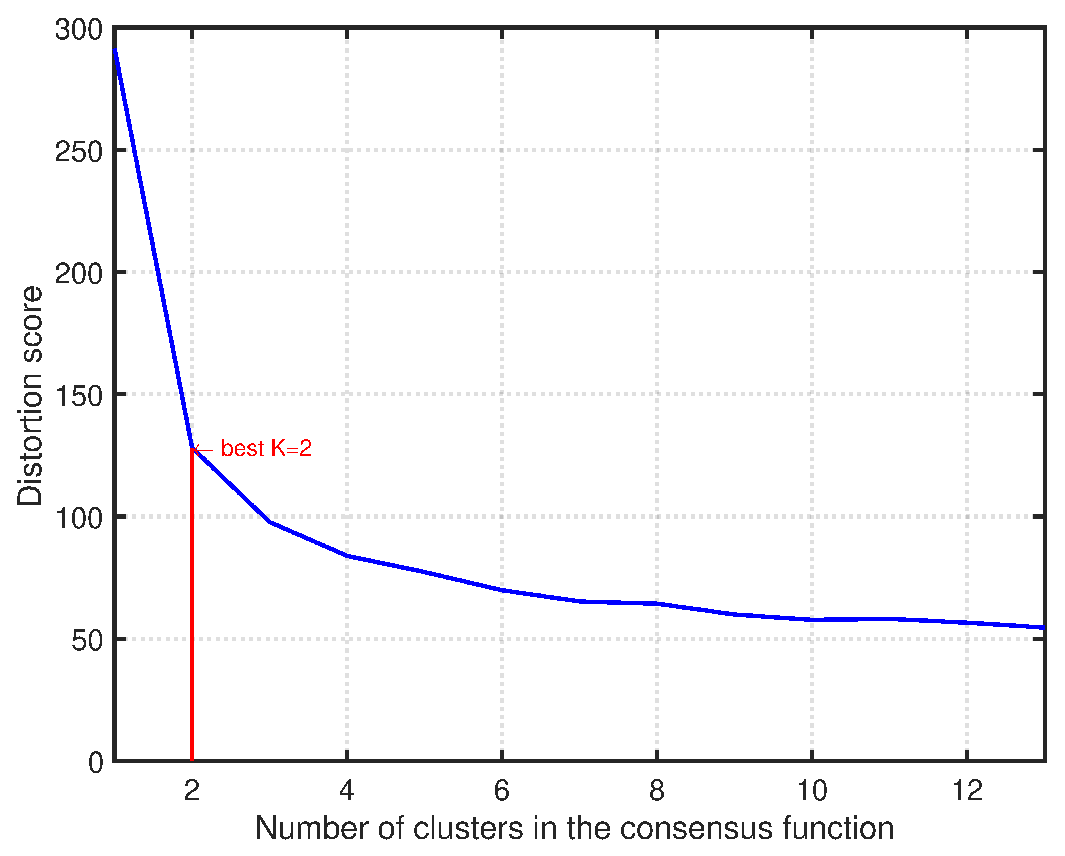
\includegraphics[width=\textwidth]{fig/iris_u_c_std_evacluster_distortionscore.eps}
  \caption{Distortion Score}
  \label{fig:iris_distortionscore}
\end{subfigure}%
\hspace*{1mm}
\begin{subfigure}[t]{0.32\textwidth}
  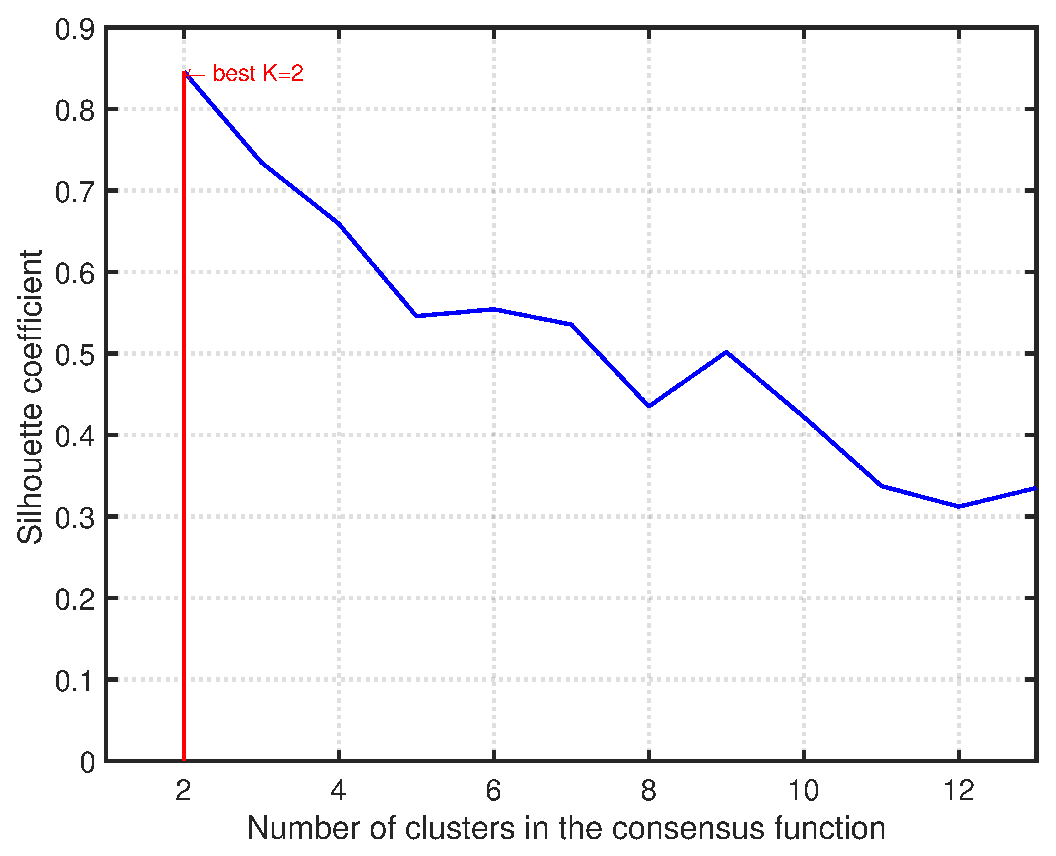
\includegraphics[width=\textwidth]{fig/iris_u_c_std_evacluster_silhouettecoefficient.eps}
  \caption{Silhouette Coefficient}
  \label{fig:iris_silhouettecoefficient}
\end{subfigure}%
\hspace*{1mm}
\begin{subfigure}[t]{0.32\textwidth}
  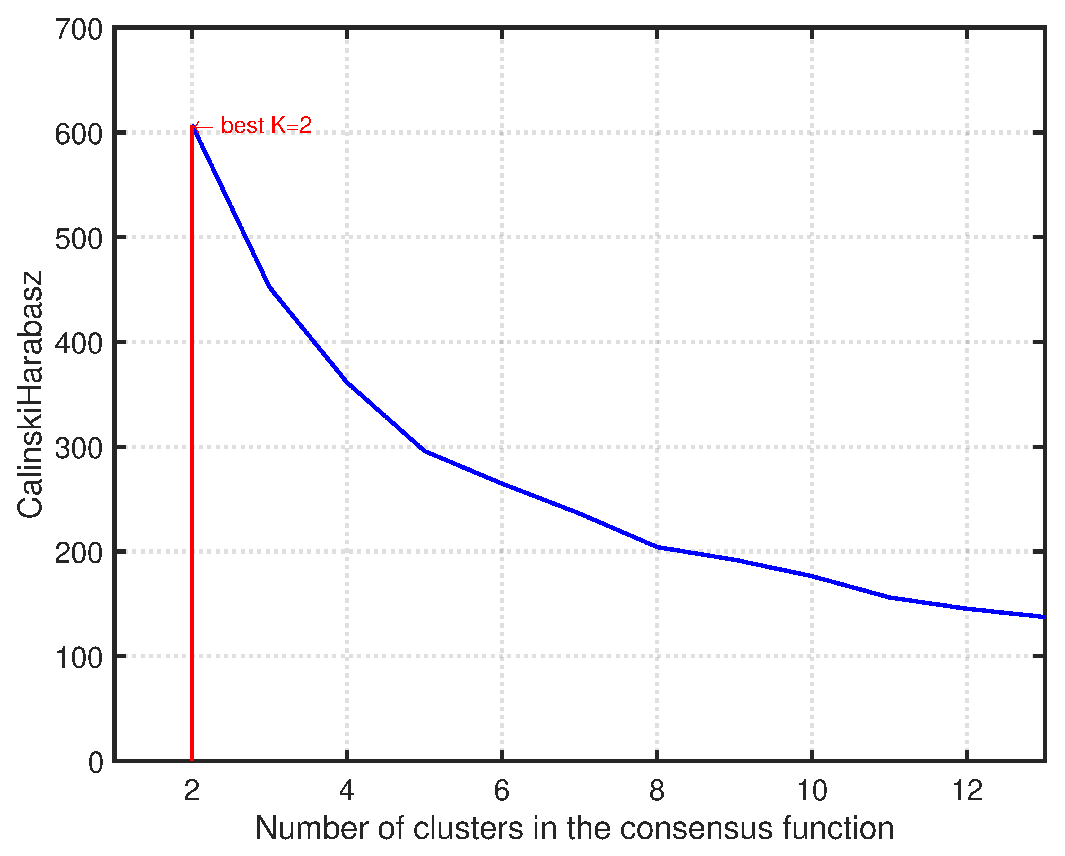
\includegraphics[width=\textwidth]{fig/iris_u_c_std_evacluster_CH.eps}
  \caption{Calinski and Harabasz index}
  \label{fig:iris_ch}
\end{subfigure}%
\caption{Impact of number of clusters in the consensus partition on the \textit{iris} data set.}
\label{fig:kimpact} % \label should be placed after \caption
\end{figure*}

\textcolor{blue}{Automatically determining the best number of clusters is another important need for the \package{KCC} package in practical clustering applications. The \package{KCC} package provides a demonstration script \textbf{Matlab/Drivers/demoEvacluster.m} for this purpose. The script is mainly composed of the following steps. The first step is to utilize three internal metrics (i.e., Distortion Score, Silhouette Coefficient, and Calinski and Harabasz index) to evaluate the quality of clustering results produced by KCC with varying number of clusters. Take the \textit{iris} data set as an example, we show the results in Figure~\ref{fig:kimpact}. As can be seen, on the iris data set, all three internal metrics generally decrease with the increase of $K$. The next step involves a selection process to find the best $K$ based on the curve of each metric in Figure~\ref{fig:kimpact}. For Distortion Score, the Elbow method~\cite{bholowalia2014ebk} is used to pick the elbow point of the curve as the the best $K$. For Silhouette Coefficient, we choose the best $K$ that produces a clustering solution with the maximum value of average silhouette coefficient. For Calinski and Harabasz index, we choose the best $K$ that produces a clustering solution with the maximum value of Calinski and Harabasz index. As indicated by the red line in Figure~\ref{fig:kimpact}, all three methods consistently find the best number of clusters as $K=2$ on the \textit{iris} data set. The most important code snippet is shown below for this illustration.}
\begin{lstlisting}[caption={Using \function{demoEvacluster.m} to determine the best number of clusters for \package{KCC}.},label=lst:findbestk]
MaxK = ceil(sqrt(size(data, 1))); % max number of clusters to choose from
distortions=zeros(MaxK, 1); % vectors storing the Distortion value for each K
silhouettes=zeros(MaxK, 1); % vectors storing the Silhouette value for each K
chs=zeros(MaxK, 1);
executiontimes=zeros(MaxK, 1); % vectors storing the execution time of running KCC
for K=1:MaxK % for each K
    tic; % record started computation time in seconds
    [pi_sumbest,pi_index,~,~~,~~~] = RunKCC(IDX,K,U,w,rep,maxIter,minThres,utilFlag);
    t = toc;
    [Distortion, Silhouette, CH] = inMeasure(data, pi_index, K);
    distortions(K,1) = Distortion;
    silhouettes(K,1) = Silhouette;
    chs(K,1) = CH;
    executiontimes(K,1)=t;
end
\end{lstlisting}

% \subsection{An illustrative example of generating basic partitions with RFS}\label{subsec:example3}
% For example, on \textit{ecoli} data set, we can generate a basic partition with $d=2$ as in the code snippet shown in Listing~\ref{lst:bpstrategy}.
% The full script for illustrating this study is in \textbf{Matlab/Drivers/demoStrategyBP.m}.
% \begin{lstlisting}[caption={Using \function{BasicCluster\_RFS} to generate BPs.},label=lst:bpstrategy]
% IDX = BasicCluster_RFS(data, 100, 6, 'sqEuclidean', 2);
% \end{lstlisting}

% \subsection{An illustrative example of generating different number of basic partitions}\label{subsec:example4}
% Taking the data set \textit{breast\_w} with $r=10$ as an example, we can execute the code snippet as in Listing~\ref{lst:numberbp} to generate a subset of the original basic partition matrix, i.e., \parameter{newIDX}, which is used as the input to the consensus function. The results are visualized in Figure~\ref{fig:bpimpact} using the \Matlab{} built-in \function{boxplot} function. The full script for illustrating this study is in \textbf{Matlab/Drivers/demoNumberBP.m}.
% \begin{lstlisting}[caption={Using \function{randsample} to generate a subset of BPs.},label=lst:numberbp]
% r = 10;
% IDX = BasicCluster_RPS(data, 1000, 2, 'sqEuclidean', 1);
% newIDX = IDX(:, randsample(1000, r));
% \end{lstlisting}

% \subsection{An illustrative example of generating incomplete basic partitions}\label{subsec:example5}
% For example, with Strategy-I on \textit{breast\_w}, we generate incomplete basic partitions with $rr=10 \%$ as indicated in Listing~\ref{lst:ibpstrategy1}. 
% Full code snippets of experiments with Strategy-I and Strategy-II is in \textbf{Matlab/Drivers/demoIBPI.m} and \textbf{Matlab/Drivers/demoIBPII.m}, respectively.
% \begin{lstlisting}[caption={Using Strategy-I to generate IBPs.},label=lst:ibpstrategy1]
% rr = 0.1;
% IDX = BasicCluster_RPS_missing(data, 100, 2, 'sqEuclidean', 1, rr);
% \end{lstlisting}

% For Strategy-II on \textit{breast\_w}, we generate incomplete basic partitions with $rr=10 \%$ as indicated in Listing~\ref{lst:ibpstrategy2}.
% \begin{lstlisting}[caption={Using Strategy-II to generate IBPs.},label=lst:ibpstrategy2]
% rr = 0.1;
% IDX = BasicCluster_RPS(data, 100, 2, 'sqEuclidean', 1);
% newIDX = addmissing(IDX, rr);
% \end{lstlisting}

\section{Matlab functions that are provided to the user}\label{sec:functions}
In this section, we give the details of each function, including brief description of the function, syntax of invoking the function, input parameters, output parameters, and a discussion regarding the important details of the function.

\subsection{BasicCluster\_RFS}
This function generates basic partition results using $K$-means as a basic clustering algorithm with Random Feature Selection (RFS) strategy.

\syntax{IDX = BasicCluster\_RFS(Data, r, K, dist, nFeature)}

\begin{inputlist}
  \paramitem{Data}{input data matrix}
  \paramitem{r}{the predefined number of basic partitions in the cluster ensemble}
  \paramitem{K}{the predefined number of clusters in the basic partitions}
  \paramitem{dist}{the distance measure used in $K$-means clustering}
  \paramitem{nFeature}{the number of randomly selected partial features}
\end{inputlist}

\begin{outputlist}
  \paramitem{IDX}{a matrix indicating the cluster labels for data points in basic partitions}
\end{outputlist}

\begin{remark}
\noindent The parameter \texttt{Data} is an \textsf{n} $\times$ \textsf{p} matrix of data, whose rows correspond to \textsf{n} observations, and columns correspond to \textsf{p} features. The available options of the parameter \texttt{dist} can be found from the official documentation of the \Matlab{} \textsf{kmeans} function, and the most widely used distance metric is \texttt{`sqEuclidean'}, which denotes the squared Euclidean distance. For \texttt{`sqEuclidean'}, the centroid for each cluster is calculated as the mean of the data points in that cluster. For selecting features, we first sample \textsf{nFeature} values uniformly at random without replacement from the integers \textsf{1} to \textsf{p}, where \textsf{p} is the dimension of all features in the input data. Then the sampled values are used as the indices of the selected features. The output \texttt{IDX} is a \textsf{n} $\times$ \textsf{r} cluster labels matrix for \textsf{n} data points in \textsf{r} basic partitions. Note that this function is a non-deterministic function. Each call may yield a different output matrix IDX, due to the random feature sampling process, and the random initializations in the $K$-means algorithm. 
\end{remark}

\subsection{BasicCluster\_RPS}
This function generates basic partition results using $K$-means as a basic clustering algorithm with Random Parameter Selection (RPS) strategy.

\syntax{IDX = BasicCluster\_RPS(Data, r, K, dist, randKi)}

\begin{inputlist}
  \paramitem{Data}{input data matrix}
  \paramitem{r}{the predefined number of basic partitions in the cluster ensemble}
  \paramitem{K}{the groundtruth number of clusters for the input data}
  \paramitem{dist}{the distance measure used in $K$-means clustering}
  \paramitem{randKi}{the parameter regarding the number of clusters in the basic partitions}
\end{inputlist}

\begin{outputlist}
  \paramitem{IDX}{a \textsf{n} $\times$ \textsf{r} cluster labels matrix for \textsf{n} data points in \textsf{r} basic partitions}
\end{outputlist}

\begin{remark}
\noindent The parameter \texttt{K} indicates the groundtruth number of clusters for the input data, which is used as the lower bound of the randomized number of cluster for each basic partition when \texttt{randKi == 1}. The parameter \textsf{randKi} has the following options. If \texttt{randKi == 1}, this function generates a random number of cluster ranging from \texttt{K} to \texttt{sqrt(n)}, where $n$ is the number of input data instances; if \texttt{randKi} is set to a \textsf{r} $\times$ \textsf{1} vector, this function produces \textsf{r} basic partitions of which the $i$-th BP's number of clusters is \textsf{RandKi(i)}; otherwise, this function produces \textsf{r} basic partitions with each partition having equal number (i.e., \textsf{K}) of clusters. Note that this function is a non-deterministic function. Each call may yield a different output matrix IDX, due to the random parameter selection process, and the random initializations in the $K$-means algorithm.
\end{remark}

\subsection{Preprocess}
This function conduct some preprocessing on the input basic partition matrix \texttt{IDX} to produce the input for the final consensus clustering, as well as some auxiliary output variables that can help to save memory and accelerate computations.

\syntax{Ki, sumKi, binIDX, missFlag, missMatrix, distance, Pvector, weight = \\ Preprocess(IDX, U, n, r, w, utilFlag)}

\begin{inputlist}
  \paramitem{IDX}{the input basic partition matrix}
  \paramitem{U}{the parameter regarding the chosen utility function}
  \paramitem{n}{the number of data instances}
  \paramitem{r}{the number of basic partitions in the cluster ensemble}
  \paramitem{w}{the weight vector for all basic partitions}
  \paramitem{utiFlag}{whether to calculate utility function}
\end{inputlist}

\begin{outputlist}
  \paramitem{Ki}{a row vector indicating the number of clusters in all basic partitions}
  \paramitem{sumKi}{a matrix indicating the starting indexes for all basic partitions}
  \paramitem{binIDX}{a sparse representation of binarization of \textsf{IDX}}
  \paramitem{missFlag}{whether the input \textsf{IDX} matrix contains IBPs or not}
  \paramitem{missMatrix}{indices matrix of the non-zero entries in \textsf{IDX} if there exists IBPs}
  \paramitem{distance}{the distance function corresponding to a specific utility function}
  \paramitem{Pvector}{a row vector calculated from the contingency matrix}
  \paramitem{weight}{an adjusted weight vector adapted for convenient distance calculation}
\end{outputlist}

\begin{remark}
\noindent The parameter \textsf{U} is a \textsf{1} $\times$ \textsf{3} cell array. Its first cell \textsf{U\{1,1\}} defines the chosen type of the KCC utility function. It currently supports four different types of utility functions which correspond to four different $K$-means point-to-centroid distance functions, i.e., \textsf{`U\_c'} for Euclidean distance, \textsf{`U\_H'} for Kullback-Leibler Divergence, \textsf{`U\_cos'} for cosine similarity, and \textsf{`U\_Lp'} for Lp-norm. It is worth noting that \textsf{`U\_Lp'} corresponds the distance measure in $L_p$ spaces, which are function spaces defined using a natural generalization of the $p$-norm for finite-dimensional vector spaces. The second cell \textsf{U\{1,2\}} is a parameter specifying the chosen form of the KCC utility function, i.e., \textsf{`std'} for the Standard Form, and \textsf{`norm'} for the Normalized Form. The third cell \textsf{U\{1,3\}} is only required to be set when \textsf{`U\_Lp'} is chosen as the utility function. The settings of \textsf{p = 1}, \textsf{p = 2}, \textsf{p} $\rightarrow \infty$ correspond to the Manhattan distance, the euclidean distance and the chebyshev distance, respectively.  The parameter \texttt{w} is \textsf{r} $\times$ \textsf{1} weight vector, of which each entry indicates the weight value assigned to each basic partition in the optimization objective of consensus clustering. The parameter \texttt{utiFlag} is a variable indicating whether to calculate utility function during the iterative process of $K$-means clustering.

\noindent The output variable \textsf{missFlag} $\in \{0, 1\}$ indicates whether the input \textsf{IDX} matrix contains incomplete basic partitions (IBPs) or not. The output \textsf{missMatrix} is a mask matrix which represents the indices of the non-zero entries in \textsf{IDX} if there exists IBPs. The output variable \textsf{distance} determines the corresponding distance function to deal with the specific utility function defined by \textsf{U\{1,1\}}. The output vector \textsf{Pvector} is a \textsf{1} $\times$ \textsf{r} row vector calculated from the contingency matrix, i.e., $P^{(i)}_k$, which can later be used in calculating distance and utility functions. The output vector \textsf{weight} is a \textsf{r} $\times$ \textsf{1} adjusted weight vector adapted for convenient distance calculation in later $K$-means heuristic. 
\end{remark}

\subsection{KCC}
This function employs the $K$-means heuristic to generate a final consensus partition.

\syntax{sumbest, index, converge, utility = KCC(IDX, K, U, w, weight, distance, \\ maxIter, minThres, utilFlag, missFlag, missMatrix, n, r, Ki, sumKi, binIDX, Pvector)}

\begin{inputlist}
  \paramitem{IDX}{the input basic partition matrix}
  \paramitem{K}{the number of clusters in the consensus partition}
  \paramitem{U}{the parameter regarding the chosen utility function}
  \paramitem{w}{the weight vector for all basic partitions}
  \paramitem{weight}{an adjusted weight vector adapted for convenient distance calculation}
  \paramitem{distance}{the distance function corresponding to a specific utility function}
  \paramitem{maxIter}{the maximum number of iterations for the convergence}
  \paramitem{minThres}{the minimum reduced threshold of objective function}
  \paramitem{utiFlag}{whether to calculate utility function}
  \paramitem{missFlag}{whether there exist IBPs in \textsf{IDX}}
  \paramitem{missMatrix}{the indices matrix of the non-zero entries in \textsf{IDX} if there exists IBPs}
  \paramitem{n}{the number of data points}
  \paramitem{r}{the number of basic partitions in the cluster ensemble}
  \paramitem{Ki}{a row vector indicating the number of clusters in all basic partitions}
  \paramitem{sumKi}{a matrix indicating the starting indexes for all basic partitions}
  \paramitem{binIDX}{a sparse representation of binarization of \textsf{IDX}}
  \paramitem{Pvector}{a row vector calculated from the contingency matrix}
\end{inputlist}

\begin{outputlist}
  \paramitem{sumbest}{the optimal value of the consensus clustering's objective function}
  \paramitem{index}{the label vector for the final consensus partition}
  \paramitem{converge}{the iterative values of objective function}
  \paramitem{utility}{the final utility function value}
\end{outputlist}

\begin{remark}
\noindent For convenience of computation, \textsf{KCC} function achieves the consensus clustering under four different conditions, e.g., (a) utility calculation is enabled and there are missing values (\textsf{utilFlag==1 \&\& missFlag==1}); (b) utility calculation is enabled and there are no missing values (\textsf{utilFlag==1 \&\& missFlag==0}); (c) utility calculation is disabled and there are missing values (\textsf{utilFlag==0 \&\& missFlag==1}); (d) utility calculation is disabled and there are no missing values (\textsf{utilFlag\\==0 \&\& missFlag==0}). Notably, we introduce a parameter called utilFlag in the KCC function to control whether the K-means heuristic computes the value of the KCC utility function, since the value of the KCC utility function might be of interest to some users in using the package. The users can choose to the enable or disable the computation of the value of the KCC utility function since it does not affect the process of K-means heuristic. Disabling the computation of the value of the KCC utility function does not affect the clustering performance and can accelerate the computation of KCC. We have added more elaborations on the usage of the parameter utilFlag in the function KCC in the user manual.
\end{remark}


\subsection{distance\_euc}
This function performs point-to-centroid distance calculation using euclidean distance measure.

\syntax{D = distance\_euc(U, C, weight, n, r, K, sumKi, binIDX)}

\begin{inputlist}
  \paramitem{U}{the \textsf{1} $\times$ \textsf{3} utility parameter cell array}
  \paramitem{C}{the centroid matrix}
  \paramitem{weight}{an \textsf{r} $\times$ \textsf{1} adjusted weight vector}
  \paramitem{n}{the number of data points}
  \paramitem{r}{the predefined number of basic partitions in the cluster ensemble}
  \paramitem{K}{the predefined number of clusters in the consensus partition}
  \paramitem{sumKi}{a matrix indicating the starting indexes for all basic partitions}
  \paramitem{binIDX}{a sparse representation of binarization of \textsf{IDX}}
\end{inputlist}

\begin{outputlist}
  \paramitem{D}{an \textsf{n} $\times$ \textsf{K} point-to-centroid distance matrix}
\end{outputlist}

\subsection{distance\_cos}
This function performs point-to-centroid distance calculation using cosine distance measure.

\syntax{D = distance\_cos(U, C, weight, n, r, K, sumKi, binIDX)}

\begin{inputlist}
  \paramitem{U}{the \textsf{1} $\times$ \textsf{3} utility parameter cell array}
  \paramitem{C}{the centroid matrix}
  \paramitem{weight}{an \textsf{r} $\times$ \textsf{1} adjusted weight vector}
  \paramitem{n}{the number of data points}
  \paramitem{r}{the predefined number of basic partitions in the cluster ensemble}
  \paramitem{K}{the predefined number of clusters in the consensus partition}
  \paramitem{sumKi}{a matrix indicating the starting indexes for all basic partitions}
  \paramitem{binIDX}{a sparse representation of binarization of \textsf{IDX}}
\end{inputlist}

\begin{outputlist}
  \paramitem{D}{an \textsf{n} $\times$ \textsf{K} point-to-centroid distance matrix}
\end{outputlist}


\subsection{distance\_kl}
This function performs point-to-centroid distance calculation using KL-divergence measure.

\syntax{D = distance\_kl(U, C, weight, n, r, K, sumKi, binIDX)}

\begin{inputlist}
  \paramitem{U}{the \textsf{1} $\times$ \textsf{3} utility parameter cell array}
  \paramitem{C}{the centroid matrix}
  \paramitem{weight}{an \textsf{r} $\times$ \textsf{1} adjusted weight vector}
  \paramitem{n}{the number of data points}
  \paramitem{r}{the predefined number of basic partitions in the cluster ensemble}
  \paramitem{K}{the predefined number of clusters in the consensus partition}
  \paramitem{sumKi}{a matrix indicating the starting indexes for all basic partitions}
  \paramitem{binIDX}{a sparse representation of binarization of \textsf{IDX}}
\end{inputlist}

\begin{outputlist}
  \paramitem{D}{an \textsf{n} $\times$ \textsf{K} point-to-centroid distance matrix}
\end{outputlist}


\subsection{distance\_lp}
This function performs point-to-centroid distance calculation using $L_p$ norm measure.

\syntax{D = distance\_lp(U, C, weight, n, r, K, sumKi, binIDX)}

\begin{inputlist}
  \paramitem{U}{the \textsf{1} $\times$ \textsf{3} utility parameter cell array}
  \paramitem{C}{the centroid matrix}
  \paramitem{weight}{an \textsf{r} $\times$ \textsf{1} adjusted weight vector}
  \paramitem{n}{the number of data points}
  \paramitem{r}{the predefined number of basic partitions in the cluster ensemble}
  \paramitem{K}{the predefined number of clusters in the consensus partition}
  \paramitem{sumKi}{a matrix indicating the starting indexes for all basic partitions}
  \paramitem{binIDX}{a sparse representation of binarization of \textsf{IDX}}
\end{inputlist}

\begin{outputlist}
  \paramitem{D}{an \textsf{n} $\times$ \textsf{K} point-to-centroid distance matrix}
\end{outputlist}


\subsection{distance\_euc\_miss}
This function performs point-to-centroid distance calculation over data with IBPs using euclidean distance measure.

\syntax{D = distance\_euc\_miss(U, C, weight, n, r, K, sumKi, binIDX, missMatrix)}

\begin{inputlist}
  \paramitem{U}{the \textsf{1} $\times$ \textsf{3} utility parameter cell array}
  \paramitem{C}{the centroid matrix}
  \paramitem{weight}{an \textsf{r} $\times$ \textsf{1} adjusted weight vector}
  \paramitem{n}{the number of data points}
  \paramitem{r}{the predefined number of basic partitions in the cluster ensemble}
  \paramitem{K}{the predefined number of clusters in the consensus partition}
  \paramitem{sumKi}{a matrix indicating the starting indexes for all basic partitions}
  \paramitem{binIDX}{a sparse representation of binarization of \textsf{IDX}}
  \paramitem{missMatrix}{the indices matrix of the non-zero entries in \textsf{IDX} if there exists IBPs}
\end{inputlist}

\begin{outputlist}
  \paramitem{D}{an \textsf{n} $\times$ \textsf{K} point-to-centroid distance matrix}
\end{outputlist}


\subsection{distance\_cos\_miss}
This function performs point-to-centroid distance calculation over data with IBPs using cosine distance measure.

\syntax{D = distance\_cos\_miss(U, C, weight, n, r, K, sumKi, binIDX, missMatrix)}

\begin{inputlist}
  \paramitem{U}{the \textsf{1} $\times$ \textsf{3} utility parameter cell array}
  \paramitem{C}{the centroid matrix}
  \paramitem{weight}{an \textsf{r} $\times$ \textsf{1} adjusted weight vector}
  \paramitem{n}{the number of data points}
  \paramitem{r}{the predefined number of basic partitions in the cluster ensemble}
  \paramitem{K}{the predefined number of clusters in the consensus partition}
  \paramitem{sumKi}{a matrix indicating the starting indexes for all basic partitions}
  \paramitem{binIDX}{a sparse representation of binarization of \textsf{IDX}}
  \paramitem{missMatrix}{the indices matrix of the non-zero entries in \textsf{IDX} if there exists IBPs}
\end{inputlist}

\begin{outputlist}
  \paramitem{D}{an \textsf{n} $\times$ \textsf{K} point-to-centroid distance matrix}
\end{outputlist}


\subsection{distance\_kl\_miss}
This function performs point-to-centroid distance calculation over data with IBPs using KL-divergence measure.

\syntax{D = distance\_kl\_miss(U, C, weight, n, r, K, sumKi, binIDX, missMatrix)}

\begin{inputlist}
  \paramitem{U}{the \textsf{1} $\times$ \textsf{3} utility parameter cell array}
  \paramitem{C}{the centroid matrix}
  \paramitem{weight}{an \textsf{r} $\times$ \textsf{1} adjusted weight vector}
  \paramitem{n}{the number of data points}
  \paramitem{r}{the predefined number of basic partitions in the cluster ensemble}
  \paramitem{K}{the predefined number of clusters in the consensus partition}
  \paramitem{sumKi}{a matrix indicating the starting indexes for all basic partitions}
  \paramitem{binIDX}{a sparse representation of binarization of \textsf{IDX}}
  \paramitem{missMatrix}{the indices matrix of the non-zero entries in \textsf{IDX} if there exists IBPs}
\end{inputlist}

\begin{outputlist}
  \paramitem{D}{an \textsf{n} $\times$ \textsf{K} point-to-centroid distance matrix}
\end{outputlist}


\subsection{distance\_lp\_miss}
This function performs point-to-centroid distance calculation over data with IBPs using $L_p$ norm measure.

\syntax{D = distance\_lp\_miss(U, C, weight, n, r, K, sumKi, binIDX, missMatrix)}

\begin{inputlist}
  \paramitem{U}{the \textsf{1} $\times$ \textsf{3} utility parameter cell array}
  \paramitem{C}{the centroid matrix}
  \paramitem{weight}{a \textsf{r} $\times$ \textsf{1} adjusted weight vector}
  \paramitem{n}{the number of data points}
  \paramitem{r}{the number of basic partitions in the cluster ensemble}
  \paramitem{K}{the predefined number of clusters}
  \paramitem{sumKi}{a matrix indicating the starting indexes for all basic partitions}
  \paramitem{binIDX}{the sparse representation matrix}
  \paramitem{missMatrix}{the indices matrix of the non-zero entries in \textsf{IDX} if there exists IBPs}
\end{inputlist}

\begin{outputlist}
  \paramitem{D}{an \textsf{n} $\times$ \textsf{K} point-to-centroid distance matrix}
\end{outputlist}


\subsection{UCompute}
This function performs utility calculation on data sets without missing values.

\syntax{util =  UCompute(index, U, w, C, n, r, K, sumKi, Pvector)}

\begin{inputlist}
  \paramitem{index}{an \textsf{n} $\times$ \textsf{1} cluster assignment matrix}
  \paramitem{U}{the \textsf{1} $\times$ \textsf{3} utility parameter cell array}
  \paramitem{w}{the \textsf{r} $\times$ \textsf{1} adjusted weight parameter vector}
  \paramitem{C}{the centroid matrix}
  \paramitem{n}{the number of data points}
  \paramitem{r}{the number of basic partitions in the cluster ensemble}
  \paramitem{K}{the predefined number of clusters in the consensus partition}
  \paramitem{sumKi}{a matrix indicating the starting indexes for all basic partitions}
  \paramitem{Pvector}{a \textsf{1} $\times$ \textsf{r} row vector calculated from the contingency matrix}
\end{inputlist}

\begin{outputlist}
  \paramitem{util}{the utility values calculated from the optimization objective of consensus clustering}
\end{outputlist}

\begin{remark}
\noindent The output \texttt{util} is a \textsf{2} $\times$ \textsf{1} cell array including a utility gain and an adjusted utility value.
\end{remark}


\subsection{UCompute\_miss}
This function performs utility calculation on data sets with missing values.

\syntax{util =  UCompute\_miss(index, U, w, C, n, r, K, sumKi, Pvector, M)}

\begin{inputlist}
  \paramitem{index}{an \textsf{n} $\times$ \textsf{1} cluster assignment matrix}
  \paramitem{U}{the \textsf{1} $\times$ \textsf{3} utility parameter cell array}
  \paramitem{w}{the \textsf{r} $\times$ \textsf{1} adjusted weight parameter vector}
  \paramitem{C}{the centroid matrix}
  \paramitem{n}{the number of data points}
  \paramitem{r}{the number of basic partitions in the cluster ensemble}
  \paramitem{K}{the predefined number of clusters in the consensus partition}
  \paramitem{sumKi}{a matrix indicating the starting indexes for all basic partitions}
  \paramitem{Pvector}{a \textsf{1} $\times$ \textsf{r} row vector calculated from the contingency matrix}
  \paramitem{M}{a mask matrix indicating the indices of the non-zero entries in \textsf{IDX}}
\end{inputlist}

\begin{outputlist}
  \paramitem{util}{the utility values calculated from the optimization objective of consensus clustering}
\end{outputlist}


\subsection{RunKCC}
This function combines the two functions, i.e., \textsf{Preprocess} and \textsf{KCC}, for finding the consensus partition in one step.

\syntax{[pi\_sumbest, pi\_index, pi\_converge, pi\_utility, t] = RunKCC(IDX, K, U, w, rep, maxIter, minThres, utilFlag)}

\begin{inputlist}
  \paramitem{IDX}{the basic partition matrix}
  \paramitem{K}{the predefined number of clusters in the consensus partition}
  \paramitem{U}{the \textsf{1} $\times$ \textsf{3} utility parameter cell array}
  \paramitem{w}{the \textsf{r} $\times$ \textsf{1} adjusted weight parameter vector}
  \paramitem{rep}{the number of repeated KCC experiments for selecting the best result}
  \paramitem{maxIter}{the maximum number of iterations for the convergence}
  \paramitem{minThres}{the minimum reduced threshold of objective function}
  \paramitem{utiFlag}{whether to calculate utility function}
\end{inputlist}

\begin{outputlist}
  \paramitem{pi\_sumbest}{the value of objective function for the best KCC experiment}
  \paramitem{pi\_index}{the cluster assignment matrix in the consensus partition for the best KCC experiment}
  \paramitem{pi\_converge}{the iterative values of objective function for the best KCC experiment}
  \paramitem{pi\_utility}{the utility values for the best KCC experiment}
  \paramitem{t}{the execution time cost of the whole process for this function}
\end{outputlist}

\subsection{exMeasure}
This function assesses the clustering quality of the results obtained by a clustering algorithm with external validity indices.

\syntax{[Acc, Rn, NMI, VIn, VDn, labelnum, ncluster, cmatrix] = exMeasure(cluster, true\_label)}

\begin{inputlist}
  \paramitem{cluster}{a \textsf{n} $\times$ \textsf{1} cluster assignment matrix returned by a clustering algorithm}
  \paramitem{true\_label}{the true class labels for the data points}
\end{inputlist}

\begin{outputlist}
  \paramitem{Acc}{the classification accuracy}
  \paramitem{Rn}{the normalized Rand statistic}
  \paramitem{NMI}{the normalized mutual information}
  \paramitem{VIn}{the normalized Variation of Information}
  \paramitem{VDn}{the normalized van Dongen criterion}
  \paramitem{labelnum}{the number of unique labels in the groundtruth data}
  \paramitem{ncluster}{the number of clusters returned by the algorithm}
  \paramitem{cmatrix}{a \textsf{ncluster} $\times$ \textsf{labelnum} contingency matrix}
\end{outputlist}

\begin{remark}
\noindent This function implements five external validity indices, including classification accuracy~\cite{nguyen2007consensus} ($CA$), the normalized mutual information~\cite{cover2012elements} ($NMI$), the normalized Rand statistic~\cite{rand1971objective} ($R_n$), the normalized van Dongen criterion~\cite{dongen2000performance} ($VD_n$), and the normalized Variation of Information~\cite{cover2012elements} ($VI_n$). In implementing the \textsf{exMeasure} function, we utilize a function called \textsf{bestMap} written by \cite{CHH05}, in which the Hungarian method~\cite{carpaneto1980algorithm} is employed to resolve the label assignment issue in clustering.
\end{remark}

\subsection{inMeasure}
This function assesses the clustering quality of the results obtained by a clustering algorithm with internal validity indices.

\syntax{[Distortion, Silhouette] = inMeasure(IDX, cluster, U)}

\begin{inputlist}
  \paramitem{IDX}{the input basic partition matrix for KCC}
  \paramitem{cluster}{the clustering decision matrix returned by KCC}
  \paramitem{U}{the \textsf{1} $\times$ \textsf{3} utility parameter cell array}
\end{inputlist}

\begin{outputlist}
  \paramitem{Distortion}{the distortion score}
  \paramitem{Silhouette}{the average silhouette coefficient value of all data objects}
\end{outputlist}

\begin{remark}
\noindent This function implements two internal validity indices, including Distortion Score~\cite{bradley1998refining} and Silhouette Coefficient~\cite{kaufman2009finding}. Distortion Score corresponds to the sum of the distance squared between the data objects and the centroid of their assigned cluster.
\end{remark}

% References
\begin{small}
\bibliography{references}
\bibliographystyle{ACM-Reference-Format}
\end{small}

\end{document}
